\section{How to translate}

To have all the translations working correctly two major steps are required. Repeat these two steps for each application.

\subsection{Step 1: Create a new language file}

\begin{enumerate}
    \item Go to the application's root folder
    \item Go to the folder \textbf{src/assets/i18n/} (figure \ref{fig:i18n_folder} shows an example for the AMP application). The \textbf{English.json} and \textbf{Portuguese.json} files must exist in that folder.
    \item Create a new JSON file. Name it the new language in English (ex.: \textbf{Spanish.json}). The first letter of the name must be uppercase.
    \item Copy all the contents of the \textbf{English.json} file to the new file
    \item Translate all the English sentences to the new language, except in the ``LANGUAGES'' substructure
    \item Inside the file find the ``LANGUAGES'' substructure (figure \ref{fig:languages_substructure})
    \begin{enumerate}
        \item Add your language to the substructure. The key is the name of the language in English. The value is the name of the language in the language (ex.: ``Spanish'': ``Español'')
        \item Repeat the previous step for all language files
    \end{enumerate}
\end{enumerate}

\begin{figure}[ht]
    \centering
    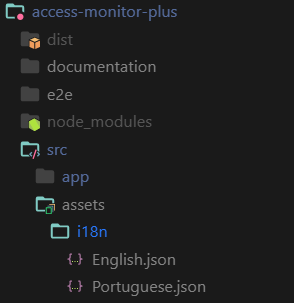
\includegraphics{lib/images/translate/i18n_folder.png}
    \caption{Language files location example}
    \label{fig:i18n_folder}
\end{figure}

\begin{figure}[ht]
    \centering
    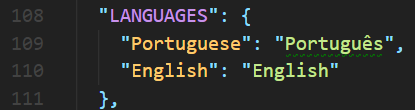
\includegraphics{lib/images/translate/languages_substructure.png}
    \caption{JSON file, ``LANGUAGES'' substructure}
    \label{fig:languages_substructure}
\end{figure}

\subsection{Step 2: Add the new language to the code}

\begin{enumerate}
    \item Go to the application's root folder
    \item Go to the folder \textbf{src/app/}
    \item Open the \textbf{app.component.ts} file
    \item Find the languages structures (figure \ref{fig:code_lang_structures})
    \item Add the language to the \textbf{langs} structure (ex.: ``es'': ``Spanish'')
    \item Add the language code to the \textbf{langCodes} structure (ex.: ``Spanish'': ``es'')
    \item Change the default language and backup language in case of missing translations (figure \ref{fig:code_default_lang})
    \begin{enumerate}
        \item In line 43 and 49 change the language \textbf{Portuguese} to the desired default language
    \end{enumerate}
    \item Go to the folder \textbf{src/} inside the application's root folder
    \item Open the \textbf{index.html} file
    \item Change the attribute \textbf{lang} from the \textbf{html} tag to the desired lang code, figure \ref{fig:html_code_default_lang}, line 2
\end{enumerate}

\begin{figure}[ht]
    \centering
    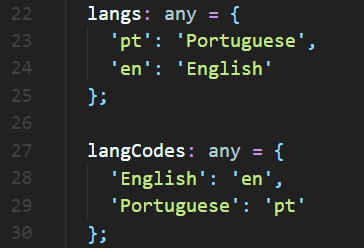
\includegraphics{lib/images/translate/code_lang_strcuture.png}
    \caption{Languages structures in the code}
    \label{fig:code_lang_structures}
\end{figure}

\begin{figure}[ht]
    \centering
    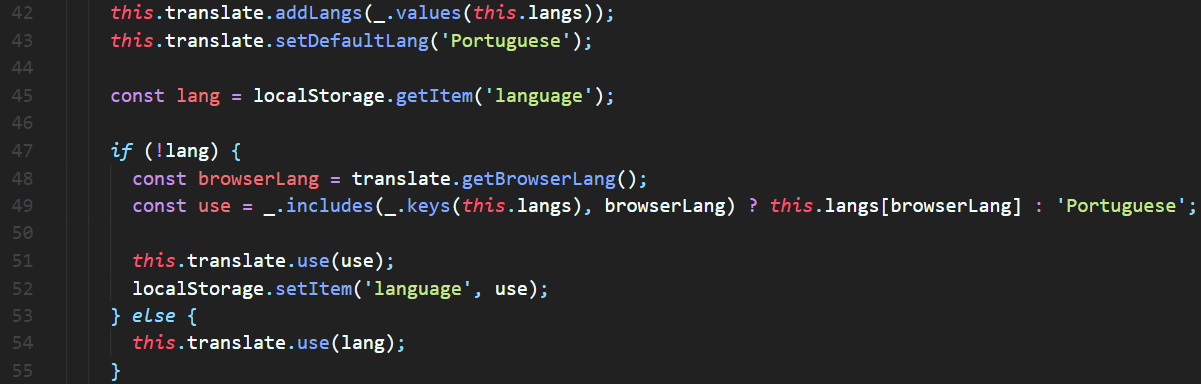
\includegraphics[width=\linewidth]{lib/images/translate/code_default_lang.png}
    \caption{Definition of the default language in the code}
    \label{fig:code_default_lang}
\end{figure}

\begin{figure}[ht]
    \centering
    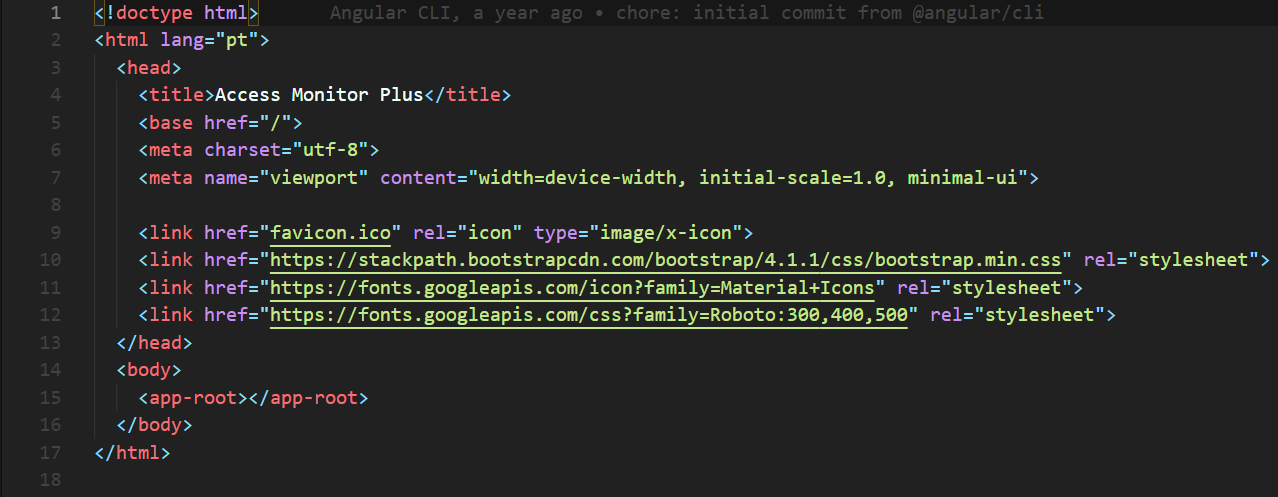
\includegraphics[width=\linewidth]{lib/images/translate/index_html_lang.png}
    \caption{Definition of the default language in the \textbf{index.html} file}
    \label{fig:html_code_default_lang}
\end{figure}